\iffalse
This file is protected by Copyright. Please refer to the COPYRIGHT file
distributed with this source distribution.

This file is part of OpenCPI <http://www.opencpi.org>

OpenCPI is free software: you can redistribute it and/or modify it under the
terms of the GNU Lesser General Public License as published by the Free Software
Foundation, either version 3 of the License, or (at your option) any later
version.

OpenCPI is distributed in the hope that it will be useful, but WITHOUT ANY
WARRANTY; without even the implied warranty of MERCHANTABILITY or FITNESS FOR A
PARTICULAR PURPOSE. See the GNU Lesser General Public License for more details.

You should have received a copy of the GNU Lesser General Public License along
with this program. If not, see <http://www.gnu.org/licenses/>.
\fi

%----------------------------------------------------------------------------------------
% Update the docTitle and docVersion per document
%----------------------------------------------------------------------------------------
\def\docTitle{OpenCPI\\Ettus E3XX Getting Started Guide}
\def\docVersion{1.3}
%----------------------------------------------------------------------------------------
\documentclass{article}
\iffalse
This file is protected by Copyright. Please refer to the COPYRIGHT file
distributed with this source distribution.

This file is part of OpenCPI <http://www.opencpi.org>

OpenCPI is free software: you can redistribute it and/or modify it under the
terms of the GNU Lesser General Public License as published by the Free Software
Foundation, either version 3 of the License, or (at your option) any later
version.

OpenCPI is distributed in the hope that it will be useful, but WITHOUT ANY
WARRANTY; without even the implied warranty of MERCHANTABILITY or FITNESS FOR A
PARTICULAR PURPOSE. See the GNU Lesser General Public License for more details.

You should have received a copy of the GNU Lesser General Public License along
with this program. If not, see <http://www.gnu.org/licenses/>.
\fi
% Any changes to this document should be made in opencpi.git
\author{} % Force author to be blank
%----------------------------------------------------------------------------------------
% Paper size, orientation and margins
%----------------------------------------------------------------------------------------
\usepackage{geometry}
\geometry{
        letterpaper, % paper type
        portrait,    % text direction
        left=.75in,  % left margin
        top=.75in,   % top margin
        right=.75in, % right margin
        bottom=.75in % bottom margin
 }
%----------------------------------------------------------------------------------------
% Header/Footer
%----------------------------------------------------------------------------------------
\usepackage{fancyhdr} \pagestyle{fancy} % required for fancy headers
\renewcommand{\headrulewidth}{0.5pt}
\renewcommand{\footrulewidth}{0.5pt}
\rhead{\small{ANGRYVIPER Team}}
% \rfoot{\thepage}
%----------------------------------------------------------------------------------------
% Appendix packages
%----------------------------------------------------------------------------------------
\usepackage[toc,page]{appendix}
%----------------------------------------------------------------------------------------
% Defined Commands & Renamed Commands
%----------------------------------------------------------------------------------------
\renewcommand{\contentsname}{Table of Contents}
\renewcommand{\listfigurename}{List of Figures}
\renewcommand{\listtablename}{List of Tables}
\newcommand{\todo}[1]{\textcolor{red}{TODO: #1}\PackageWarning{TODO:}{#1}} % To do notes
\newcommand{\code}[1]{\texttt{#1}} % For inline code snippet or command line
%----------------------------------------------------------------------------------------
% Various packages
%----------------------------------------------------------------------------------------
\usepackage[usenames,dvipsnames]{xcolor} % for color names see https://en.wikibooks.org/wiki/LaTeX/Colors
\usepackage{hyperref}  % for linking urls and lists
\usepackage{graphicx}  % for including pictures by file
\usepackage{listings}  % for coding language styles
\usepackage{rotating}  % for sideways table
\usepackage{pifont}    % for sideways table
\usepackage{pdflscape} % for landscape view
\usepackage{subfig}
\hyphenation{ANGRY-VIPER} % Tell it where to hyphenate
\hyphenation{Cent-OS} % Tell it where to hyphenate
\hyphenation{install-ation} % Tell it where to hyphenate
\uchyph=0 % Never hyphenate acronyms like RCC (I think this overrides ANGRYVIPER above)
\renewcommand\_{\textunderscore\allowbreak} % Allow words to break/newline on underscores
%----------------------------------------------------------------------------------------
% Table packages
%----------------------------------------------------------------------------------------
\usepackage{longtable} % for long possibly multi-page tables
\usepackage{tabularx} % c=center,l=left,r=right,X=fill
% These define tabularx columns "C" and "R" to match "X" but center/right aligned
\newcolumntype{C}{>{\centering\arraybackslash}X}
\newcolumntype{R}{>{\raggedleft\arraybackslash}X}
\usepackage{float}
\floatstyle{plaintop}
\usepackage[tableposition=top]{caption}
\newcolumntype{P}[1]{>{\centering\arraybackslash}p{#1}}
\newcolumntype{M}[1]{>{\centering\arraybackslash}m{#1}}
%----------------------------------------------------------------------------------------
% Block Diagram / FSM Drawings
%----------------------------------------------------------------------------------------
\usepackage{tikz}
\usetikzlibrary{shapes,arrows,fit,positioning}
\usetikzlibrary{automata} % used for the fsm
%----------------------------------------------------------------------------------------
% Colors Used
%----------------------------------------------------------------------------------------
\usepackage{colortbl}
\definecolor{blue}{rgb}{.7,.8,.9}
\definecolor{ceruleanblue}{rgb}{0.16, 0.32, 0.75}
\definecolor{drkgreen}{rgb}{0,0.6,0}
\definecolor{deepmagenta}{rgb}{0.8, 0.0, 0.8}
\definecolor{cyan}{rgb}{0.0,0.6,0.6}
\definecolor{maroon}{rgb}{0.5,0,0}
%----------------------------------------------------------------------------------------
% VHDL Coding Language Style
% modified from: http://latex-community.org/forum/viewtopic.php?f=44&t=22076
%----------------------------------------------------------------------------------------
\lstdefinelanguage{VHDL}
{
        basicstyle=\ttfamily\footnotesize,
        columns=fullflexible,keepspaces,      % https://tex.stackexchange.com/a/46695/87531
        keywordstyle=\color{ceruleanblue},
        commentstyle=\color{drkgreen},
        morekeywords={
    library,use,all,entity,is,port,in,out,end,architecture,of,
    begin,and, signal, when, if, else, process, end,
        },
        morecomment=[l]--
}
%----------------------------------------------------------------------------------------
% XML Coding Language Style
% modified from: http://tex.stackexchange.com/questions/10255/xml-syntax-highlighting
%----------------------------------------------------------------------------------------
\lstdefinelanguage{XML}
{
        basicstyle=\ttfamily\footnotesize,
        columns=fullflexible,keepspaces,
        morestring=[s]{"}{"},
        morecomment=[s]{!--}{--},
        commentstyle=\color{drkgreen},
        moredelim=[s][\color{black}]{>}{<},
        moredelim=[s][\color{cyan}]{\ }{=},
        stringstyle=\color{maroon},
        identifierstyle=\color{ceruleanblue}
}
%----------------------------------------------------------------------------------------
% DIFF Coding Language Style
% modified from http://tex.stackexchange.com/questions/50176/highlighting-a-diff-file
%----------------------------------------------------------------------------------------
\lstdefinelanguage{diff}
{
        basicstyle=\ttfamily\footnotesize,
        columns=fullflexible,keepspaces,
        breaklines=true,                                % wrap text
        morecomment=[f][\color{ceruleanblue}]{@@},      % group identifier
        morecomment=[f][\color{red}]-,                  % deleted lines
        morecomment=[f][\color{drkgreen}]+,             % added lines
        morecomment=[f][\color{deepmagenta}]{---},      % Diff header lines (must appear after +,-)
        morecomment=[f][\color{deepmagenta}]{+++},
}
%----------------------------------------------------------------------------------------
% Python Coding Language Style
% modified from
%----------------------------------------------------------------------------------------
\lstdefinelanguage{python}
{
        basicstyle=\ttfamily\footnotesize,
        columns=fullflexible,keepspaces,
        keywordstyle=\color{ceruleanblue},
        commentstyle=\color{drkgreen},
        stringstyle=\color{orange},
        morekeywords={
    print, if, sys, len, from, import, as, open,close, def, main, for, else, write, read, range,
        },
        comment=[l]{\#}
}
%----------------------------------------------------------------------------------------
% Fontsize Notes in order from smallest to largest
%----------------------------------------------------------------------------------------
%    \tiny
%    \scriptsize
%    \footnotesize
%    \small
%    \normalsize
%    \large
%    \Large
%    \LARGE
%    \huge
%    \Huge

\date{Version \docVersion} % Force date to be blank and override date with version
\title{\docTitle}
\lhead{Ettus E3XX Getting Started Guide}
%----------------------------------------------------------------------------------------
\usepackage[T1]{fontenc} % http://tex.stackexchange.com/a/181119
\usepackage{graphicx}
\graphicspath{ {figures/} }
\lstset{ % https://tex.stackexchange.com/a/116572
  basicstyle=\ttfamily,
  columns=fullflexible,
  % frame=single,
  breaklines=true,
  showstringspaces=true,
  showspaces=true,
  postbreak=\mbox{\textcolor{red}{$\hookrightarrow$}\space},
}
\begin{document}
\maketitle
\begin{figure}[H]
 \centering
 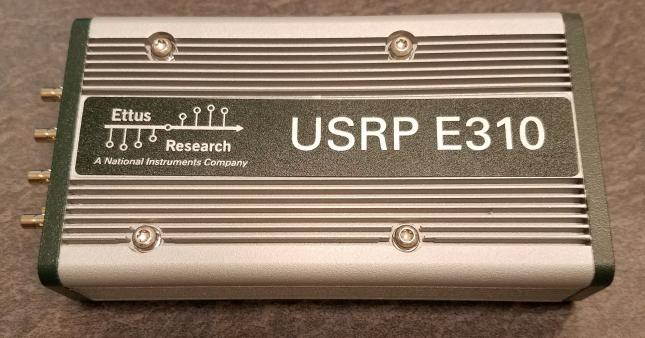
\includegraphics[scale=0.9]{img/top.jpg}
 \caption{Top View (E310)}
 \label{fig:top}
\end{figure}
%\thispagestyle{fancy}
\newpage

	\begin{center}
	\textit{\textbf{Revision History}}
		\begin{table}[H]
		\label{table:revisions} % Add "[H]" to force placement of table
			\begin{tabularx}{\textwidth}{|c|X|l|}
			\hline
			\rowcolor{blue}
			\textbf{Revision} & \textbf{Description of Change} & \textbf{Date} \\
		    \hline
		    v1.3.1-E3XX & Initial Release & 3/2018 \\
			\hline
			\end{tabularx}
		\end{table}
	\end{center}

\newpage

\tableofcontents

\newpage

\section{References}

	This document assumes a basic understanding of the Linux command line (or ``shell'') environment.  The reference(s) in Table 1 can be used as an overview of OpenCPI and may prove useful.

\def\refcapbottom{}
\iffalse
This file is protected by Copyright. Please refer to the COPYRIGHT file
distributed with this source distribution.

This file is part of OpenCPI <http://www.opencpi.org>

OpenCPI is free software: you can redistribute it and/or modify it under the
terms of the GNU Lesser General Public License as published by the Free Software
Foundation, either version 3 of the License, or (at your option) any later
version.

OpenCPI is distributed in the hope that it will be useful, but WITHOUT ANY
WARRANTY; without even the implied warranty of MERCHANTABILITY or FITNESS FOR A
PARTICULAR PURPOSE. See the GNU Lesser General Public License for more details.

You should have received a copy of the GNU Lesser General Public License along
with this program. If not, see <http://www.gnu.org/licenses/>.
\fi

% This snippet creates the "References" table labeled "table:references"
% It creates three columns: Name, Publisher, Link and then inserts default documents
%
% To skip these defaults, define macros named
% refskipgs to skip "Getting Started"
% refskipig to skip "Installation Guide"
% refskipac to skip "Acronyms and Definitions"
% refskipocpiov to skip "OpenCPI Overview"
%
% See RPM_Installation_Guide.tex for examples
%
% After the defaults, it optionally inserts the "myreferences" macro that
% you defined elsewhere (you put hlines above all lines)
%
% If you want the \caption on the bottom, define "refcapbottom"
\begin{center}
\renewcommand*\footnoterule{} % Remove separator line from footnote
\renewcommand{\thempfootnote}{\arabic{mpfootnote}} % Use Arabic numbers (or can't reuse)
\begin{minipage}{0.9\textwidth}
  \begin{table}[H]
\ifx\refcapbottom\undefined
  \caption {References}
  \label{table:references}
\fi
  \begin{tabularx}{\textwidth}{|C|c|C|}
    \hline
    \rowcolor{blue}
    \textbf{Title} & \textbf{Published By} & \textbf{Link} \\
\ifx\refskipgs\undefined
    \hline
    Getting Started & ANGRYVIPER Team & \path{Getting_Started.pdf} \\
\fi
\ifx\refskipig\undefined
    \hline
    Installation Guide & ANGRYVIPER Team & \path{RPM_Installation_Guide.pdf} \\
\fi
\ifx\refskipac\undefined
    \hline
    Acronyms and Definitions & ANGRYVIPER Team & \path{Acronyms_and_Definitions.pdf} \\
\fi
\ifx\refskipocpiov\undefined
    \hline
    Overview & OpenCPI &
% Analytics: https://goo.gl/info/RskxiV
\url{https://goo.gl/RskxiV} \\
\fi
\ifx\myreferences\undefined
\else
    \myreferences
\fi
    \hline
  \end{tabularx}
\ifx\refcapbottom\undefined
\else
  \caption {References}
  \label{table:references}
\fi
  \end{table}
\end{minipage}
\end{center}


\newpage
\section{Overview}
The purpose of this document is to provide instructions for configuring a development host to design OpenCPI software applications that target an Ettus Research/National Instruments Universal Software Radio Peripheral (USRP) E3XX SDR (\textit{e.g.} E310) and configuration of this SDR as an integrated OpenCPI platform.

\section{Prerequisites}
\subsection{OpenCPI Software Setup}
\begin{flushleft}
This guide assumes that the following RPMs are installed:  \\
\begin{table}[H]

		\label{table:rpms}
			\begin{tabularx}{\textwidth}{|C|X|}
			\hline
			\rowcolor{blue}
			\textbf{RPM Name} & \textbf{Description} \\
			\hline
			(All prerequisite RPMs compiled for the Zynq platform, \textit{e.g.} \path{ocpi-prereq-xz-platform-zynq}) & These packages have OpenCPI-specific patches and are provided as RPMs. This packaging ensures they will not conflict with other installed copies by using a nonstandard installation location of \path{/opt/opencpi/prerequisites}. \\
		    \hline
		    \path{opencpi-1.3.1-*.el7.centos.x86_64} & Base installation RPM includes the runtime portion of the Component Development Kit (CDK), scripts for creating the user's workspace, and limited documentation. \\
		    \hline
		    \path{opencpi-devel-*.el7.centos.x86_64} & Additional header files and scripts for developing new assets as HDL and/or RCC. \\
		    \hline
		    \path{opencpi-hw-platform-e3xx-*.el7.centos.noarch} & Additional files necessary to build the framework targeting the E3XX hardware platform. \\
		    \hline
		    \path{opencpi-sw-platform-xilinx13_4-*.el7.centos.noarch} & Additional files necessary to build the framework targeting the Xilinx 13.4 Linux software platform. \\
		    \hline
			\end{tabularx}
\end{table}
\subsection{Vendor Software Setup}
The SDR that is expected to be used is the Ettus Research/National Instruments Universal Software Radio Peripheral (USRP) E3XX SDR (\textit{e.g.} E310). This OpenCPI-enabled SDR provides the capability of deploying hardware and software workers while using Xilinx's 13.4 distribution of Linux; a variant of the standard distribution used by OpenCPI.\\ \bigskip

\begin{center}
\framebox{\parbox{0.8\linewidth}{\centering Note: As of this writing, the ``standard'' OSS OpenCPI uses Xilinx 13.4 (\path{xilinx13_4}). \\
The ANGRYVIPER Team's RPM-based version uses Xilinx 13.3 (\path{xilinx13_3}). \\
This means that a user cannot have a single system configured to develop for the E3XX \textit{and} any other Zynq-based platform (\textit{e.g.} \path{zed}) at the same time, because you can only have one of the \path{opencpi-sw-platform-xilinx*} RPMs installed at a time.}}
\end{center}
\ \bigskip % Gap under box

The synthesizers and cross-compilers required to build HDL and RCC Workers for this Platform are installed by following the instructions found in the \textit{OpenCPI FPGA Vendor Tools Installation Guide}. This document assumes that the user has installed the appropriate versions of Vivado and the Xilinx SDK.\\ \bigskip

\subsection{Building Required Projects}
The Core, Assets, and the E310-BSP Projects must be built \textit{in the given order} for this platform\footnote{See the ANGRYVIPER Team's Getting Started Guide for additional information concerning these other Projects and the \path{ocpidev} command.}. A specific example follows. \bigskip

\subsubsection*{Specific Example}
This example will extract the three Projects into a single location.
\begin{lstlisting}[showspaces=false]
$ mkdir <your work location>
$ cd <your work location>
$ /opt/opencpi/projects/new_project_source core core_project
$ /opt/opencpi/projects/new_project_source assets assets_project
$ /opt/opencpi/projects/new_project_source bsp_e310 bsp_e310
$ ls
assets_project  core_project  bsp_e310
$ ocpidev show projects
ocpi.assets ocpi.cdk ocpi.core ocpi.bsp.e310
<can verify paths with --table option>
$ for proj in core_project assets_project bsp_e310; do \
ocpidev -d $proj build --rcc-platform xilinx13_4; \
done
<output cut>
$ for proj in core_project assets_project; do \
ocpidev -d $proj build --hdl-platform e3xx --no-assemblies; \
done
<output cut>
$ ocpidev -d bsp_e310 --hdl-platform e3xx
<output cut>
\end{lstlisting}

\subsection{Hardware Setup}
\begin{figure}[h]
 \centering
 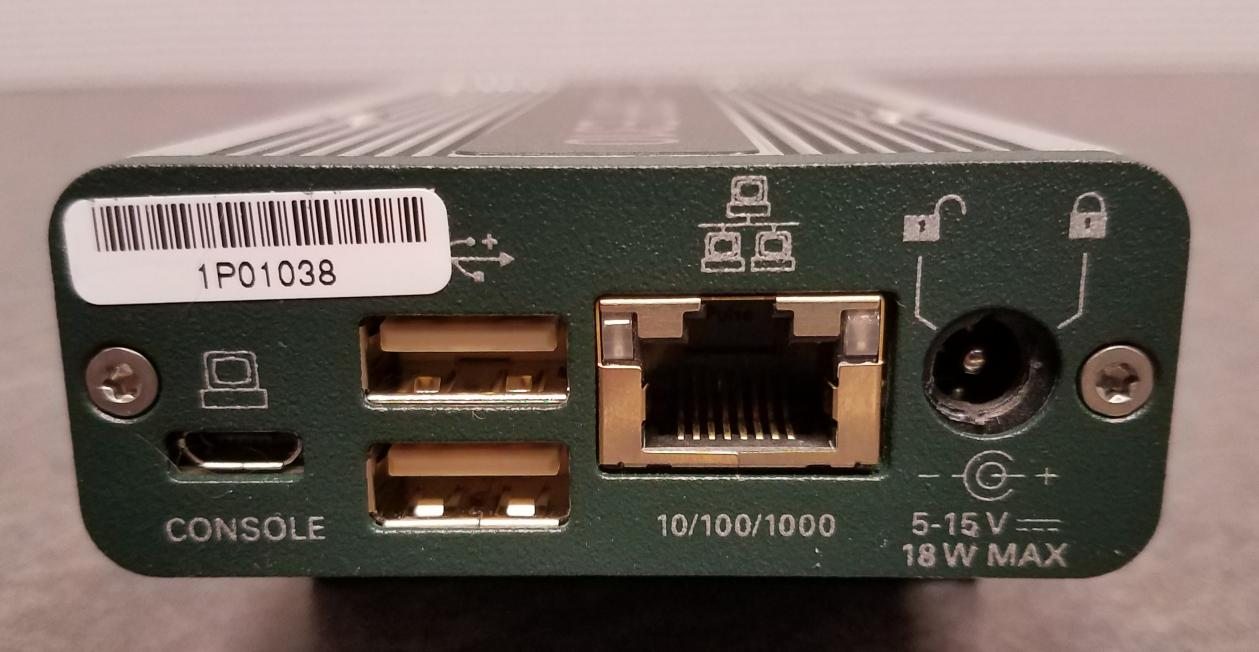
\includegraphics[scale=0.5]{img/back_panel.jpg}
 \caption{Back Panel}
 \label{fig:back}
\end{figure}

Plug an Ethernet cable into the SDR's networking port (Figure~\ref{fig:back}). The SDR obtains an IP Address by using DHCP. This is a requirement if operating in network mode (discussed in Section~\ref{sec:network_mode}). Located on the back panel is a Micro-B USB port marked ``CONSOLE'' (Figure~\ref{fig:back}), which provides a serial console interface to the embedded Linux OS (see Section~\ref{sec:serial_setup}).\\ \bigskip

\begin{figure}[h]
 \centering
 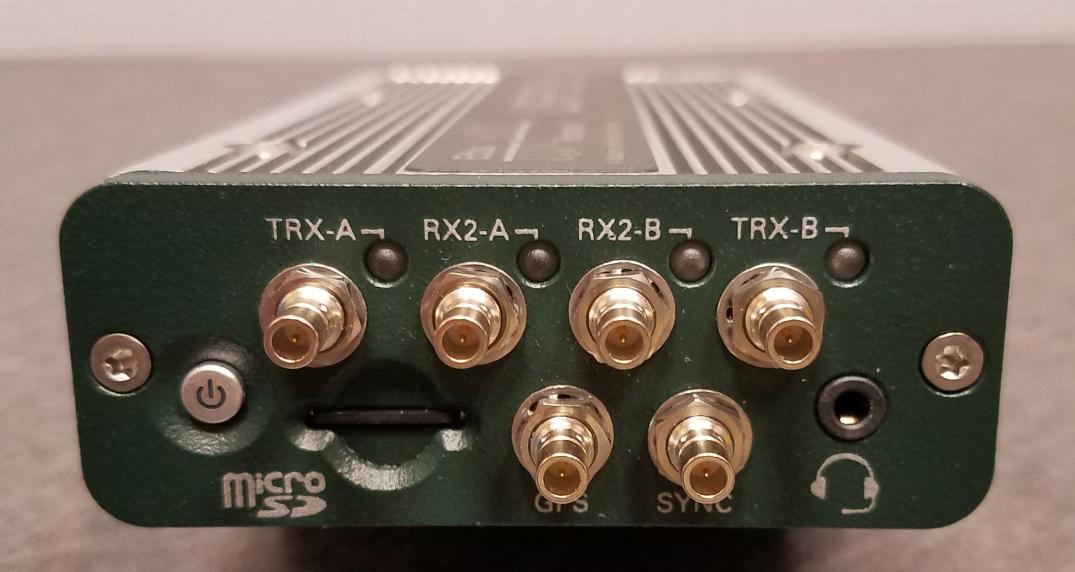
\includegraphics[scale=0.5]{img/front_panel.jpg}
 \caption{Front Panel}
 \label{fig:front}
\end{figure}

The bootable SD card slot is located on the front of the unit (Figure~\ref{fig:front}) and ejects by gently pushing it in and releasing. Also found on the front panel of the SDR are six labeled SMB (50 Ohm) connectors: TRX-A, RX2-A, RX2-B, TRX-B, GPS, and SYNC. The upper connections are split into two individual channels referred to as ``Front End A'' and ``Front End B.'' Specific details can be found in the vendor manuals. \\   \bigskip

\end{flushleft}
\section{Script Setup}
\label{sec:script}
There are two modes for running OpenCPI applications on any embedded radio: network mode and standalone mode. Network mode is when the development system hosts the OpenCPI tree as an NFS server to the embedded radio as an NFS client. This configuration provides easy and dynamic access to all of OpenCPI, and presumably any components and applications. Standalone mode is when all of the artifacts are located on the SDR's local storage (\textit{e.g.} SD card) and no network connection is required. This is a better \textit{deployment} mode, and is better for situations where a network connection is not possible or practical. Network mode is generally preferred when it is possible because it makes the development process easier than standalone mode. \\

There are separate startup scripts that are run on the SDR for each mode. These scripts will need to be modified for each user's specific setup and file structure. There are templates for these scripts that are provided by the framework found in \path{/opt/opencpi/boot_support/e3xx/OpenCPI-SD-e3xx/opencpi/}. Both \path{mynetsetup.sh} and \path{mysetup.sh} have a template file available with \path{default_} prepended there. \\

\textit{For either usage mode}, the following settings \textit{might} need to be modified:

\begin{itemize}
 \item The system to be used as a time server. Defaulted to ``\code{time.nist.gov}''. Change this if you have a local time server that supports RFC-868.
 \item The current timezone description. Defaulted to ``\code{EST5EDT,M3.2.0,M11.1.0}''.  Change this if required for the local timezone. See \texttt{man tzset} on the host PC for more information.
 \item If you do not have a time server, or cannot connect to a time server, you \textit{may} need to manually set the time at start up.  Use the \texttt{date} command to manually set the Linux system time. See \texttt{man date} on the host PC for more information. If system time is not required to be accurate, you can comment out this step.
\end{itemize}

\begin{flushleft}
\textit{When using Network Mode}, the following modifications are required:
\end{flushleft}

\begin{enumerate}
\item In \texttt{mynetsetup.sh}, find the example lines which are necessary for mounting the various Projects:\\

%\begin{lstlisting}
\verb+mount -t nfs -o udp,nolock,soft,intr $1:/home/user/e310/core_project /mnt/core_project+\\
\verb+mount -t nfs -o udp,nolock,soft,intr $1:/home/user/e310/assets_project /mnt/assets_project+
%\end{lstlisting}
\item Uncomment and edit \path{/home/user/e310/core_project} and \path{/home/user/e310/assets_project} to reflect the paths to the Core and Assets Projects on the development host \textit{and} add other Projects (\textit{e.g.} BSP Projects such as \code{bsp\_e310}) as required.\footnote{Additional setup will be required on the host and is covered in Section~\ref{sec:network_mode}.}
\end{enumerate}

\begin{flushleft}
\textit{For Standalone Mode}, all OpenCPI artifacts required to run any applications on the SDR need to be copied onto the SD card. See Section~\ref{sec:SD_Setup} for SD Card details.
\end{flushleft}

\section{SD Card Setup}
\label{sec:SD_Setup}
\subsection{Make a Backup Image of the SD Card}
This optional section provides the steps for creating an SD card backup image. The following sections assume the SD card is prepopulated from the vendor. \textit{It is recommended to use a new SD card and keep the original vendor SD in a safe location.} If you do not have the original SD card, or you have made no significant changes to the SD card, then this can be skipped and a new image can be downloaded at a later time if required; consult the vendor's \path{README}\footnote{\url{http://files.ettus.com/e3xx_images/README}} to determine which image is appropriate based upon your SDR's serial number.
\begin{enumerate}
\item Determine the device file name for the SD card. It will likely be something like \texttt{/dev/sdb} or \texttt{/dev/mmcblk0}. To do this, you can take a look at the end of dmesg: ``\texttt{dmesg | tail -n 15}''.
\item Run the command ``\texttt{dd if=DEVICENAME of=backup.image}'' where DEVICENAME was determined above. This step should take $\sim15$ minutes depending on the card size.
\item Compress a copy of the image using a file compression utility, \textit{e.g.} ``\code{xz -kv9e backup.image}''
\end{enumerate}
\noindent To later restore the card back to the original contents, run the command ``\texttt{dd of=DEVICENAME if=backup.image}''

\subsection{Formatting and Populating the SD Card}
\textit{Note:} The following commands expect the user to be proficient enough with Linux to consider specific commands used to be outside the scope of this document.
\begin{enumerate}
\item Format the SD card with a single FAT32 partition and remount it
\item Copy all of the contents of \path{/opt/opencpi/boot_support/e3xx/OpenCPI-SD-e3xx/} directory to the top level of this partition.
\item Copy your customized configuration scripts from Section~\ref{sec:script} to the partition under \path{opencpi/} (the path should already exist).
\end{enumerate}

\subsection{SDR Login}
With the SDR card inserted, the unit should now boot a valid OpenCPI environment. The user name and password for the development board are both ``\code{root}''.

\subsection{SD Card Source}
The final SD Card artifacts are distributed in \path{/opt/opencpi/boot_support/e3xx/OpenCPI-SD-e3xx/} via RPM as noted previously. The end user is not required nor expected to generate the files, but the process is documented below in Appendix~\ref{app:sd_card}.

\section{Hardware Setup}
\subsection{Serial setup}
\label{sec:serial_setup}
By default, the USB-to-serial adapter will connect to a host development box as read-only by non-\code{root} users unless \texttt{udev} rules are added to have the device connect as read/write. To connect to the SDR's console, use the command ``\code{sudo screen /dev/ttyUSB 115200}\footnote{It may come up as a different device, \textit{e.g.} \code{/dev/ttyUSB2}}'' on your host system.

\section{Host Setup}

% Bring in NFS setup snippet (has subsections)
\iffalse
This file is protected by Copyright. Please refer to the COPYRIGHT file
distributed with this source distribution.

This file is part of OpenCPI <http://www.opencpi.org>

OpenCPI is free software: you can redistribute it and/or modify it under the
terms of the GNU Lesser General Public License as published by the Free Software
Foundation, either version 3 of the License, or (at your option) any later
version.

OpenCPI is distributed in the hope that it will be useful, but WITHOUT ANY
WARRANTY; without even the implied warranty of MERCHANTABILITY or FITNESS FOR A
PARTICULAR PURPOSE. See the GNU Lesser General Public License for more details.

You should have received a copy of the GNU Lesser General Public License along
with this program. If not, see <http://www.gnu.org/licenses/>.
\fi
% Any changes to this document should be made in opencpi.git

% This is for inserting into various "Getting Started" Guides
% First, turn off indenting to avoid all the flushleft
\newlength{\savedparindentnfs}%
\setlength{\savedparindentnfs}{\parindent}%
\setlength{\parindent}{0pt} % Don't indent all paragraphs
\providecommand{\forceindent}{\leavevmode{\parindent=1em\indent}}%

\subsection{Network Mounting Mode}
\label{sec:network_mode}
The NFS server needs to be enabled on the host in order to run the SDR in Network Mode. The following sections are directions on how to do this for both CentOS~6 and CentOS~7 host operating systems.
\subsubsection{CentOS~6}
% \begin{minipage}{\linewidth}
From the host, install the necessary tools using yum:
\begin{verbatim}
% sudo yum install nfs-utils nfs-utils-lib
% sudo chkconfig nfs on
% sudo service rpcbind start
% sudo service nfs start
\end{verbatim}
% \end{minipage}
% ~\\

% \begin{minipage}{\linewidth}
From the host, add the following lines to the bottom of \texttt{/etc/exports} and change ``XX.XX.XX.XX/MM'' to a valid netmask for the DHCP range that the SDR will be set to for your network (\textit{e.g.} \texttt{192.168.0.0/16}).
\begin{verbatim}
% sudo vi /etc/exports

/opt/opencpi XX.XX.XX.XX/MM(rw,sync,no_root_squash,no_subtree_check)
<host core project location> XX.XX.XX.XX/MM(rw,sync,no_root_squash,no_subtree_check)
<host assets project location> XX.XX.XX.XX/MM(rw,sync,no_root_squash,no_subtree_check)

% sudo exportfs -av
\end{verbatim}
% \end{minipage}
% ~\\

% \begin{minipage}{\linewidth}
From the host, restart the services that have modified for the changes to take effect:
\begin{verbatim}
% sudo service nfs start
\end{verbatim}
% \end{minipage}

\subsubsection{CentOS~7}
% \begin{minipage}{\linewidth}
From the host, install the necessary tools using yum:\\
~\\
\verb+% sudo yum install nfs-utils+ \footnote{\texttt{nfs-utils-lib} was rolled into \texttt{nfs-utils} starting with CentOS 7.2, if using eariler versions of CentOS 7, \texttt{nfs-utils-lib} will need to be explicitly installed}
% \end{minipage}
~\\

% \begin{minipage}{\linewidth}
From the host, allow NFS past SELinux\footnote{You can use \texttt{getsebool} to see if these values are already set before attempting to set them. Some security tools may interpret the change attempt as a system attack.}:
\begin{verbatim}
% sudo setsebool -P nfs_export_all_rw 1
% sudo setsebool -P use_nfs_home_dirs 1
\end{verbatim}
% \end{minipage}
% ~\\

% \begin{minipage}{\linewidth}
From the host, allow NFS past the firewall:
\begin{verbatim}
% sudo firewall-cmd --permanent --zone=public --add-service=nfs
% sudo firewall-cmd --permanent --zone=public --add-port=2049/udp
% sudo firewall-cmd --permanent --zone=public --add-service=mountd
% sudo firewall-cmd --permanent --zone=public --add-service=rpc-bind
% sudo firewall-cmd --reload
\end{verbatim}
% \end{minipage}
% ~\\

% \begin{minipage}{\linewidth}
Define the export by creating a new file that has the extension ``\texttt{exports}''. If it does not have that extension, it will be ignored.  Add the following lines to that file and replace ``XX.XX.XX.XX/MM'' with a valid netmask for the DHCP range that the SDR will be set to for your network (\textit{e.g.} \texttt{192.168.0.0/16}).
\begin{verbatim}
% sudo vi /etc/exports.d/user_ocpi.exports

/opt/opencpi XX.XX.XX.XX/MM(rw,sync,no_root_squash,crossmnt)
/home/user/ocpi_projects/core XX.XX.XX.XX/MM(rw,sync,no_root_squash,crossmnt)
/home/user/ocpi_projects/assets XX.XX.XX.XX/MM(rw,sync,no_root_squash,crossmnt)
\end{verbatim}
% \end{minipage}
% ~\\

% \begin{minipage}{\linewidth}
If the file system that you are mounting is XFS, then each mount needs to have a unique \texttt{fsid} defined. Instead, use:
\begin{verbatim}
% sudo vi /etc/exports.d/user_ocpi.exports

/opt/opencpi XX.XX.XX.XX/MM(rw,sync,no_root_squash,crossmnt,fsid=33)
/home/user/ocpi_projects/core XX.XX.XX.XX/MM(rw,sync,no_root_squash,crossmnt,fsid=34)
/home/user/ocpi_projects/assets XX.XX.XX.XX/MM(rw,sync,no_root_squash,crossmnt,fsid=35)
\end{verbatim}
% \end{minipage}
% ~\\

% \begin{minipage}{\linewidth}
Restart the services that have modified for the changes to take effect:
\begin{verbatim}
% sudo systemctl enable rpcbind
% sudo systemctl enable nfs-server
% sudo systemctl enable nfs-lock
% sudo systemctl enable nfs-idmap
% sudo systemctl restart rpcbind
% sudo systemctl restart nfs-server
% sudo systemctl restart nfs-lock
% sudo systemctl restart nfs-idmap
\end{verbatim}
% \end{minipage}
% ~\\

* Note: Some of the ``enable'' commands may fail based on your package selection, but should not cause any problems.
\setlength{\parindent}{\savedparindentnfs}%

%

\section{Using the SDR in Network Mode}
\begin{flushleft}
Every time the SDR is rebooted, the user is required to run the \texttt{mynetsetup.sh} script, which configures the system for OpenCPI with support for network/NFS mode. The user passes the network address of the development system host in as the only argument to \texttt{mynetsetup.sh}. If the radio complains that ``No IP address was detected,'' double check your network connection and reboot the radio.\bigskip

After the SDR is booted, the first thing that needs to be done is to source the \texttt{mynetsetup.sh} script with\\
\leavevmode{\parindent=3em\indent}\code{. /mnt/card/opencpi/mynetsetup.sh XX.XX.XX.XX} \\
and changing XX.XX.XX.XX to the IP address of the NFS host (your development machine, \textit{e.g.} 192.168.1.10).
\end{flushleft}

\section{Using the SDR in Standalone Mode}
\begin{flushleft}
All artifacts for any applications or tests that need to be located on the SD card must be in the \texttt{opencpi/artifacts} folder.  All of the helper utilities such as \texttt{ocpirun} and \texttt{ocpihdl} are already located on the SD card and do not need to be copied over to the SDR platform. \bigskip

Every time the SDR is rebooted, the user is required to run the \path{/mnt/card/mysetup.sh} script, which configures the system for OpenCPI. Any time that a new version of OpenCPI is released, the SD card will need to be recreated in order to update the artifacts and the executables that are stored on the SD card.
\end{flushleft}

\iffalse
\todo{bias xml example here like ZedBoard does}
\fi
\section{Running an Application}
Now that you have set up OpenCPI and the E310 radio, you can run one of the reference applications. Navigate to \code{bsp\_e310/applications/FSK} or \code{bsp\_e310/applications/rx\_app} and follow the instructions in the corresponding document (\textit{FSK\_app.pdf} and \textit{FSK\_App\_Getting\_Started\_Guide.pdf}, or \textit{RX\_app.pdf}).
\newpage

\begin{appendices}
\section{Generating Boot Artifacts}
\label{app:sd_card}
In normal use cases, the SD card should be able to be created and used as described previously in Section~\ref{sec:SD_Setup}. This section outlines the steps required to regenerate the artifacts used in those previous sections for solely informational purposes and is not expected for users to have to complete these steps.
\subsection{BOOT.bin and u-boot.img}
The original first and second stage bootloader artifacts that come installed on the E310 SD card are not suitable for the Petalinux build OpenCPI uses for its software platform as those artifacts are expecting a uImage kernel with a separate filesystem partition, while the Petalinux build uses a separate ramdisk image file. The \path{BOOT.bin} and \path{u-boot.img} files were rebuilt in order to support booting into this style of Linux images from Ettus's and Xilinx's repositories. In summary, the repositories were cloned and checked out to the proper branch, according to the release for the e310 and the bitbake recipe, and subsequently cross-compiled for ARM using the Xilinx toolchain. The steps are shown below.
\begin{lstlisting}[showspaces=false]
$ git clone https://github.com/EttusResearch/meta-ettus.git
$ cd meta-ettus && git checkout e300-daisy && cd ..
$ git clone https://github.com/Xilinx/u-boot-xlnx.git
$ cd u-boot-xlnx && git checkout 664820b231b129552e963e1a96b45ac7196ccc81 && cd ..
$ cp meta-ettus/e300-bsp/recipes-bsp/u-boot/ettus-e300/* u-boot-xlnx/
$ cd u-boot-xlnx
$ mv ps7_init.{c,h} board/xilinx/zynq/
$ git apply 0001-E300-Uses-UART0-for-console.patch
$ git apply 0002-E300-Disable-QSPI.patch
$ git apply 0003-Read-mac-address-from-i2c-EEPROM.patch
$ git apply 0001-e300-Added-memory-test.patch
$ source {xilinx-install-dir}/Xilinx/SDK/2013.4/settings64.sh
$ make zynq_zc70x_config CROSS_COMPILE=arm-xilinx-linux-gnueabi-
$ make CROSS_COMPILE=arm-xilinx-linux-gnueabi-
\end{lstlisting}
\subsection{devicetree.dtb}
The device tree needed to be modified in order to register the hardware devices with the correct hardware device driver in the Petalinux kernel. In summary, the device tree provided by Ettus was decompiled to a device tree source (\path{dts}) file using the device tree compiler (\path{dtc}), modified the text file by adding the proper "compatible" strings to the devices, and subsequently compiled back into a device tree blob (\path{dtb}). The steps shown below assume \path{dtc} is in your \path{$PATH} and the original device tree blob is in the current working directory.
\begin{lstlisting}[showspaces=false]
$ dtc -I dtb -O dts -o devicetree.dts uImage-zynq-e31x-3.dtb
$ vim devicetree.dts
$ dtc -I dts -O dtb -o devicetree.dtb devicetree.dts
\end{lstlisting}
Note: The full source for the modified devicetree.dts can be found at
\path{<BSP project>/hdl/platforms/e3xx/sd_card_source/devicetree.dts}

\subsection{uImage and uramdisk.image.gz}
The \path{uImage} and \path{uramdisk.image.gz} image files come directly from the default 13\_4 OpenCPI software platform. The 13\_3 software platform could not be used due to the SD card driver in 13\_3 not supporting the E310's SD card device.
\end{appendices}

\end{document}
